\documentclass[english,DIV=13]{scrreprt}
%\documentclass[english,DIV=13]{scrartcl}

\usepackage[utf8x]{inputenc}
\usepackage[T1]{fontenc}
\usepackage{lmodern}
\usepackage[binary-units=true]{siunitx}
% Color
% cfr http://en.wikibooks.org/wiki/LaTeX/Colors
\usepackage{color}
\usepackage[usenames,dvipsnames,svgnames,table]{xcolor}
\definecolor{dkgreen}{rgb}{0.25,0.7,0.35}
\definecolor{dkred}{rgb}{0.7,0,0}
\usepackage{graphicx}
\usepackage{url}
\usepackage{tikz}
\usepackage{pgfplots}
\usepackage{microtype}
\usepackage{xspace}

\usepackage{hyperref}
\usepackage{todonotes}
\usepackage{epstopdf}

\usepackage{multirow}
\usepackage{tabularx} % tabular with automatic line-break
\newcolumntype{Y}{>{\centering\arraybackslash}X} % centered column

\newcommand{\matlab}{\textsc{Matlab}}

% Math symbols
\usepackage{amsmath}
\usepackage{amssymb}
\usepackage{amsthm}
\DeclareMathOperator*{\argmin}{arg\,min}
\DeclareMathOperator*{\argmax}{arg\,max}

% Unit vectors
\usepackage{esint}
\usepackage{esvect}
\newcommand{\kmath}{k}
\newcommand{\xunit}{\hat{\imath}}
\newcommand{\yunit}{\hat{\jmath}}
\newcommand{\zunit}{\hat{\kmath}}
\newcommand{\uunit}{\hat{\umath}}

% Elec
\newcommand{\B}{\vec B}
\newcommand{\E}{\vec E}
\newcommand{\EMF}{\mathcal{E}}
\newcommand{\perm}{\varepsilon} % permittivity

\newcommand{\bigoh}{\mathcal{O}}
\newcommand\eqdef{\triangleq}

\DeclareMathOperator{\newdiff}{d} % use \dif instead
\newcommand{\dif}{\newdiff\!}
\newcommand{\fpart}[2]{\frac{\partial #1}{\partial #2}}
\newcommand{\ffpart}[2]{\frac{\partial^2 #1}{\partial #2^2}}
\newcommand{\fdpart}[3]{\frac{\partial^2 #1}{\partial #2\partial #3}}
\newcommand{\fdif}[2]{\frac{\dif #1}{\dif #2}}
\newcommand{\ffdif}[2]{\frac{\dif^2 #1}{\dif #2^2}}
\newcommand{\constant}{\ensuremath{\mathrm{cst}}}
\newcommand{\norm}[1]{\left\lVert#1\right\rVert}

\usepackage{babel}
% Listing
% always put it after babel
% http://tex.stackexchange.com/questions/100717/code-in-lstlisting-breaks-document-compile-error
\usepackage{listings}

% Put caption after babel
\usepackage{caption}
\usepackage{subcaption}

\definecolor{mygreen}{rgb}{0,0.6,0}
\definecolor{mygray}{rgb}{0.5,0.5,0.5}
\definecolor{mymauve}{rgb}{0.58,0,0.82}
\lstset{ %
  language=Matlab,
  backgroundcolor=\color{white},   % choose the background color; you must add \usepackage{color} or \usepackage{xcolor}
  basicstyle=\footnotesize,        % the size of the fonts that are used for the code
  breakatwhitespace=false,         % sets if automatic breaks should only happen at whitespace
  breaklines=true,                 % sets automatic line breaking
  captionpos=b,                    % sets the caption-position to bottom
  commentstyle=\color{mygreen},    % comment style
  deletekeywords={...},            % if you want to delete keywords from the given language
  escapeinside={\%*}{*)},          % if you want to add LaTeX within your code
  extendedchars=true,              % lets you use non-ASCII characters; for 8-bits encodings only, does not work with UTF-8
  frame=single,	                   % adds a frame around the code
  keepspaces=true,                 % keeps spaces in text, useful for keeping indentation of code (possibly needs columns=flexible)
  keywordstyle=\color{blue},       % keyword style
  otherkeywords={*,...},           % if you want to add more keywords to the set
  numbers=none,                    % where to put the line-numbers; possible values are (none, left, right)
  numbersep=5pt,                   % how far the line-numbers are from the code
  numberstyle=\tiny\color{mygray}, % the style that is used for the line-numbers
  rulecolor=\color{black},         % if not set, the frame-color may be changed on line-breaks within not-black text (e.g. comments (green here))
  showspaces=false,                % show spaces everywhere adding particular underscores; it overrides 'showstringspaces'
  showstringspaces=false,          % underline spaces within strings only
  showtabs=false,                  % show tabs within strings adding particular underscores
  stepnumber=2,                    % the step between two line-numbers. If it's 1, each line will be numbered
  stringstyle=\color{mymauve},     % string literal style
  tabsize=2,	                   % sets default tabsize to 2 spaces
  title=\lstname                   % show the filename of files included with \lstinputlisting; also try caption instead of title
}

\KOMAoptions{DIV=last}




% Definition to put a bar under a letter/word (to use with matrix)
\usepackage{accents}
\newcommand{\ubar}[1]{\underaccent{\bar}{#1}}
\newcommand{\uvec}[1]{\ubar{#1}}
\newcommand{\umatrix}[1]{\ubar{\ubar{#1}}}

\titlehead{}
\subject{LINMA 1731 --- Stochastic processes}
\title{Bearings-only tracking problem}
\subtitle{}
\author{\begin{tabular}{cc}
	\textsc{Cassiers} Gaëtan  & 	$33741300$ \\
	\textsc{Losseau} Bruno 	&	$78861100$
	 \end{tabular}}
\date{\today}
\publishers{}

\begin{document}
\maketitle


\tableofcontents


%Q1
\chapter{Basics}
\section*{Deriving $\umatrix{F}$ and $\uvec{U}$}

One starst by studying the making of a discretization of a movemement process in 1D, with the
variable $x(t)$. If one denotes $x_k = x(Tk)$ (with $T$ a given discretization step), one gets
\begin{align*}
    x_{k+1} &= x_k + T\dot{x}_k + \int_{Tk}^{T(k+1)}\int_{Tk}^{t}\ddot{x}(t)\dif t\dif t' \\
    \dot{x}_{k+1} &=  \dot{x}_k + \int_{Tk}^{T(k+1)}\ddot{x}(t)\dif t.
\end{align*}
This is a simple discrete-time state model, making the consideration that the terms which depends of
the integral of $\ddot{x}$
are an input signal.
One can then generalize this equation to the relative state vector $\uvec{x} = \uvec{x}^t - \uvec{x}^o$ :
\[\uvec{x}_{k+1} = \umatrix{F}\uvec{x}_k - \uvec{U}_{k,k+1} + \uvec{\epsilon}_k\]
with
\begin{itemize}
    \item The matrix
        \[\umatrix{F} =
        \begin{pmatrix}
            1 & 0 & T & 0 \\
            0 & 1 & 0 & T \\   
            0 & 0 & 1 & 0 \\
            0 & 0 & 0 & 1   
        \end{pmatrix}
        \]
    \item $\uvec{\epsilon}_k$ the variation of position and of velocity of the target caused by the
acceleration of the target,
    \item $\uvec{U}_{k,k+1}$ the variation of position and velocity of
the observer caused by the acceleration of the observer.
\end{itemize}

\section*{Deriving $h(\ubar{x})$}
Following its definition given in the statement and using the notation $\uvec{x}(i)$
for the $i$-th element of the vector $\uvec{x}$ :
\begin{align*}
    h(\uvec{x}_k) &= \mathrm{atan2}(\uvec{x}_k(1), \uvec{x}_k(2)) \\
    &= \begin{cases}
        \arctan\frac{\uvec{x}_k(1)}{\uvec{x}_k(2)} & \text{if $\uvec{x}_k(2) > 0$} \\
        \arctan\frac{\uvec{x}_k(1)}{\uvec{x}_k(2)}+\pi & \text{if $\uvec{x}_k(2) < 0$ and $\uvec{x}_k(1) \geq 0$} \\
        \arctan\frac{\uvec{x}_k(1)}{\uvec{x}_k(2)}-\pi & \text{if $\uvec{x}_k(2) < 0$ and $\uvec{x}_k(1) < 0$} \\
        0 & \text{if $\uvec{x}_k(2) \geq 0$ and $\uvec{x}_k(1) = 0$} \\
        \pi & \text{if $\uvec{x}_k(2) < 0$ and $\uvec{x}_k(1) = 0$}
    \end{cases}
\end{align*}

%Q2
\chapter{Simple model}
At first, without implementing any command, it is asked to simulate the system for $k=200$ steps, changing
the values of the variance $\sigma^2_{\theta}$ of the gausian noise on the bearing $w_k$  and
the variance  $\sigma^2_a$ of the gausian noise on the acceleration $\epsilon_k$.

\section*{Code}
For each chapter, one only presents the code that is strictly relevant. The scripts and functions 
used to plot the required results (herein \texttt{plot\_q2.m} and \texttt{gen\_plot2.m})
can be found in the linked archive. To obtain the results for all the questions, simply launch
the script \texttt{main.m}.\\

\lstinputlisting[caption={Simulating the system}]{../matlab_report/q2.m}

Every time a code uses a parameter given in the statement, it calls the following function : 
\lstinputlisting[caption={Parameters given in the statement}]{../matlab_report/gen_parameters.m}

\section*{Results}
\begin{itemize}
\item varying $\sigma_\theta$ with $\sigma_a=0$
\begin{center}	
\includegraphics[width=0.66\textwidth]{img/q2_1.eps}
\end{center}
When there is no noise, one verifies that as the relative velocity is constant and there is no error on
the bearing, the angle is constant and the the relative position is linear.\\
As the acceleration is by default equal to zero and that there is no noise on the acceleration, as the velocity is
constant, the trajectory is for all $\sigma_{\theta}$ the same.\\
Concerning the angle, the more one raises $\sigma_{\theta}$ the higher the error on the mesured angle is.

\item varying $\sigma_a$ with $\sigma_\theta=0$
\begin{center}
\includegraphics[width=0.66\textwidth]{img/q2_2.eps}
\end{center}
The more the noise on the acceleration increases, the more the trajectory is impacted. \\
In this case, the bearing is also impacted, it seems logical as one has changed the state equations :
the noise on the acceleration does change the relative position, therefore modyfing the true bearing. \\
From these comments, one could explain the situation stating that $\sigma_a$ represents the prediction of the 
change of acceleration of the target. The change of acceleration induces a change of position,
therefrom a change on the bearing.


\item varying $\sigma_\theta$ proportionaly to $\sigma_a$
\begin{center}
\includegraphics[width=0.66\textwidth]{img/q2_3.eps}
\end{center}
The higher $\sigma_a$ is set, the quicker the relative distance augments. Taking a look at the bearing,
        we observe two trends : a slow (low frequency) variation, due to the acceleration of the target
         (which is integrated twice to get the bearing, therefore the variations are slow), and 
         a high frequency variation due to the measurement errors (that are adding a white noise).

\item  Keeping $\sigma_\theta$ and $\sigma_a$ constant

\begin{center}
 \includegraphics[width=0.66\textwidth]{img/q2_4.eps}
\end{center}
When $\sigma_a=0.5$ we observe that the target motion changes reasonably slowly, and
with $\sigma_{\theta}=0.1$ the mesurement noise is not adding too much uncertainty on the bearing. \\
With three simulations, one observes the randomness of the process.
\end{itemize}



%Q3
\chapter{Building a sequential Monte Carlo algorithm}
\section*{Code}
For all the methods that use a Monte Carlo algorithm, one built a general function 
\texttt{particle\_filter.m}, based on the reference document given in the statement
\footnote{A. Srivastava. Computational methods in statistics. Florida State University, 2009.
\url{http://stat.fsu.edu/~anuj/pdf/classes/CompStatII10/BOOK.pdf}}.\\
\lstinputlisting[caption={General Monte Carlo algorithm},label={MonteCarlo}]{../matlab_report/particle_filter.m}
The main code used here is the function \texttt{q3.m} (to employ it with the proper
parameters, plot and save the results one can launch the script \texttt{plot\_q3.m}).
\newpage
\lstinputlisting[caption={Comparing the results with Monte Carlo algorithm and the model}]{../matlab_report/q3.m}
\section*{Results}
By ploting the histograms of the distribution of the points used in the Monte Carlo algorithm, 
with $\sigma_a=0.1$ and $\sigma_{\theta}=0.1$, at the beginning (k=1) one has a look alike gaussian
distibution for both the X position and Y position. The more k augments, the less the
distribution looks like a gaussian and the wider is its variance (1 when k=1, to 50 for k=200).
This indicates that the quality of the estimation decreases when $k$ augments.

\begin{center}
   \includegraphics[width=0.49\textwidth]{img/q3_hist_1.eps}
   \includegraphics[width=0.49\textwidth]{img/q3_hist_50.eps}
   \includegraphics[width=0.49\textwidth]{img/q3_hist_100.eps}
   \includegraphics[width=0.49\textwidth]{img/q3_hist_200.eps}
\end{center}


\begin{center}
	\begin{minipage}{.6\textwidth}
		\includegraphics[width=0.95\textwidth]{img/q3_path.eps}
	\end{minipage}%
	\begin{minipage}{.4\textwidth}
		Plotting the real vs. the estimated position and indicating with dots the (X,Y) of the 
		herein produced histograms (k=1,50,100,200), one sees that the more $k$ increases
		the further the estimation is from the real position. The bearing is measured at each step (with a small error) and
		one can check that the result on the angle is convincing. Yet concerning the distance the measures don't bring
		much relevant information. What helps the best is the variability of the bearing, yet it is not enough. For this
		reason the distance is quite approximative.
	\end{minipage}
\end{center}

%Q4
\chapter{Applying the Monte Carlo algorithm to an artificial submarine 
tracking problem}
\section*{Code}

As the fourth and fifth questions are both established on applying the algorithm~\ref{MonteCarlo}
to the submarine tracking problem, one decided to group the main code for questions 4 and 5
in the function \texttt{q4q5.m}.\\
\lstinputlisting[caption={The artificial submarine tracking problem initialised with 'data.m'},label={q4q5}]{../matlab_report/q4q5.m}
To call \texttt{q4q5} in the present case, one should use \texttt{q4.m} (to use it with the proper parameters,
plot and save the results one can launch the script \texttt{plot\_q4.m}).\\
\lstinputlisting[caption={Question 4}]{../matlab_report/q4.m}

\section*{Results}
To introduce the results, one uses the following legends\\

	\begin{minipage}{.5\textwidth}
		\flushleft For the positions :\\
		 \center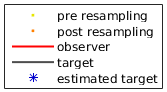
\includegraphics[width=4cm]{img/q4_legend1.png}
	\end{minipage}%
	\begin{minipage}{.3\textwidth}
		For the velocities :\\
		 \center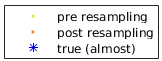
\includegraphics[width=4cm]{img/q4_legend2.png}
	\end{minipage}

\begin{itemize}
\item $k=1$\\
The distribution of the velocity particles corresponds to the initial distribution ($k=0$) : as one doesn't have yet 2 measures 
of position of the target, it cannot estimate properly the velocity and the clouds have a large scope.\\
Concerning the cloud of position particles, as one doesn't know the distance but only the bearing, it forms a shape
that is close to a line. One can easily check by extending the "line" to the initial position of the observer that it 
follows the bearing.\\
There is no big difference between the pre-resampling and the post-resampling because the initial distribution already corresponds
to the observation that is made.\\
The position and the velocity clouds are not influenced one by another : they mainly depend of the distributions that were
used to generate them at the begininng.

\item $k=2$\\
The pre-resampling position is now affected by the velocity cloud of the previous step : each pre-resampling particle position
at $k=2$ is equal to the positon at $k=1$ to which is added the velocity at $k=1$ times the time step, therefrom the cloud forms
a circular shape. As one knows the bearing (with a small error indeed), the observations makes the post-resampling cloud
in a shape that is again close to a line. Compared to $k=1$ the scope of the line is narrowed. \\
As for the velocity clouds, the pre-resampling at $k=2$ is close to the post-resampling at $k=1$. 
Now that one disposes of two positions, the velocity can be better identified : the post-resampling cloud
at $k=2$ is shrinked. \\
At this step, velocity and position have affected one another.






\begin{center}
	\begin{minipage}{.5\textwidth}
		 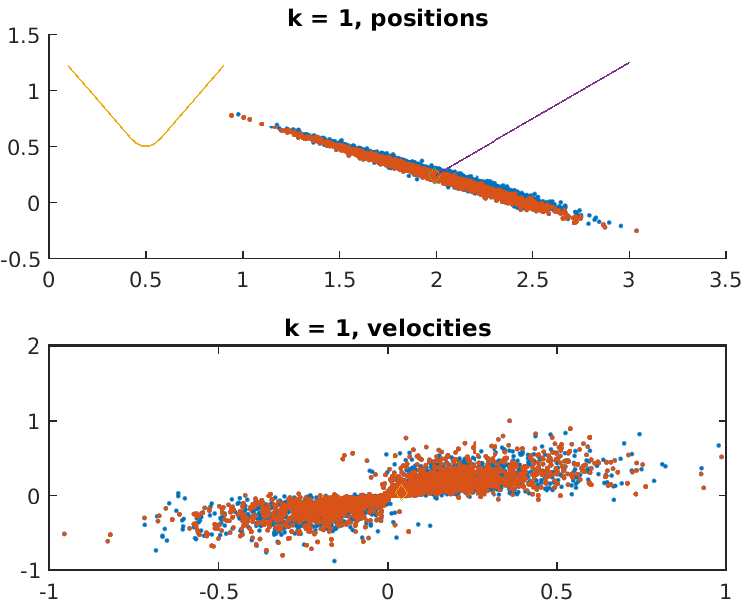
\includegraphics[width=.98\textwidth]{img/q4_1.png}
	\end{minipage}%
	\begin{minipage}{.5\textwidth}
		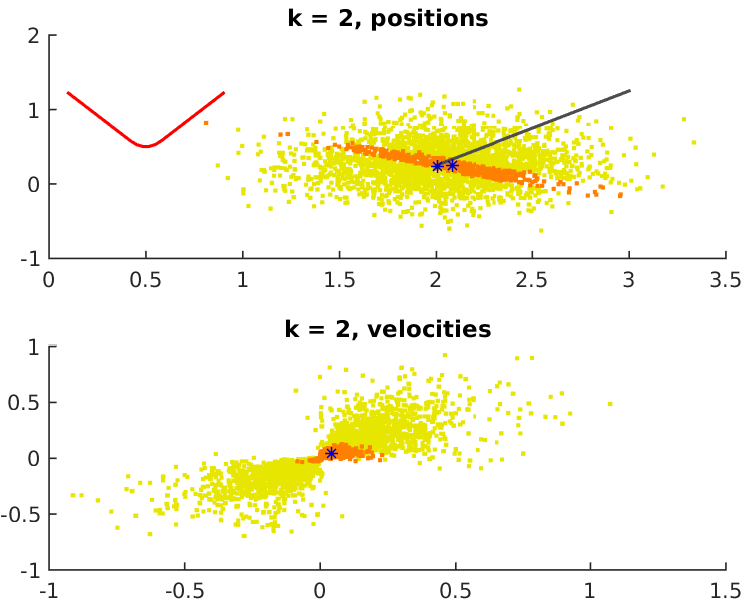
\includegraphics[width=0.98\textwidth]{img/q4_2.png}
	\end{minipage}
\end{center}
\item $k=3$\\
Concerning the position, one can observe that the post-resampling cloud is translated following the course of the target compared
to the pre-resampling cloud. Also, the bearing is increasing.\\
As for the velocity, the particle cloud stays narrow for both the pre and post-resampling.

\item $k=15$\\
The position of the observer is distinctive : it has just changed its direction. Concerning the bearing,
it has changed sign. The clouds are properly oriented, in accordance with the bearing.\\
The velocity clouds are converging : compared to $k=3$ the range of the particles is divided by a factor of order 10.

  \begin{center}
	\begin{minipage}{.5\textwidth}
   		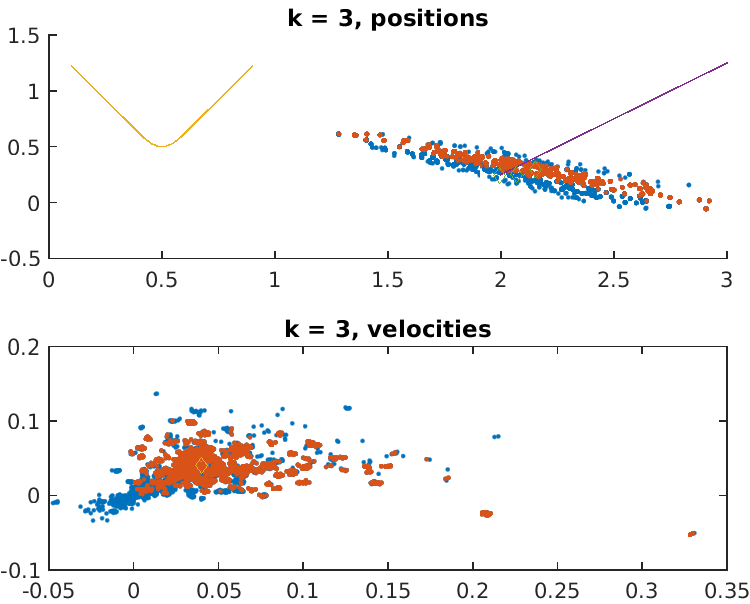
\includegraphics[width=0.98\textwidth]{img/q4_3.png}
	\end{minipage}%
	\begin{minipage}{.5\textwidth}
		 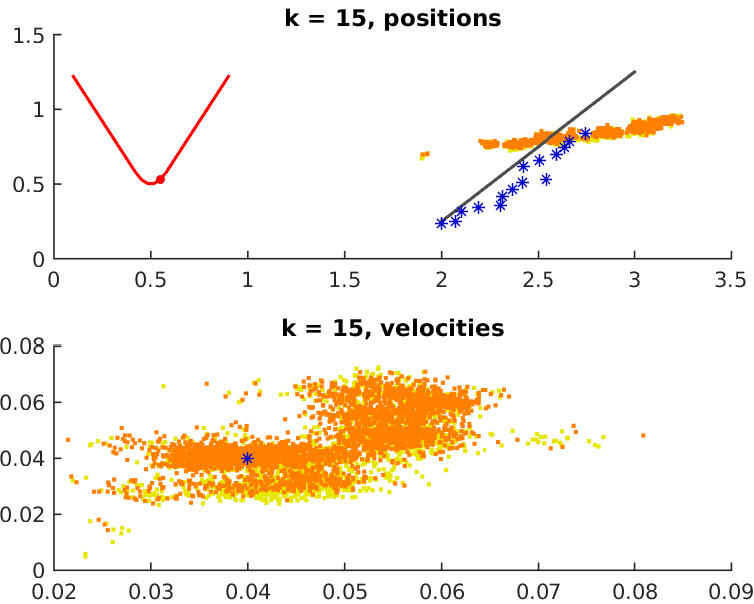
\includegraphics[width=0.98\textwidth]{img/q4_15.png}
	\end{minipage}
\end{center}
\item $k=26$\\
In the end, one still has a line shape for the pre and post-resampling clouds, its length hasn't much decreased
since $k=3$. This is still due to the fact that one has the observation on the bearing but not on the distance.
Hence the bearing is still correct.\\
Since $k=15$, there hasn't been any improvement in the range of the velocity clouds.

  \begin{center}
		 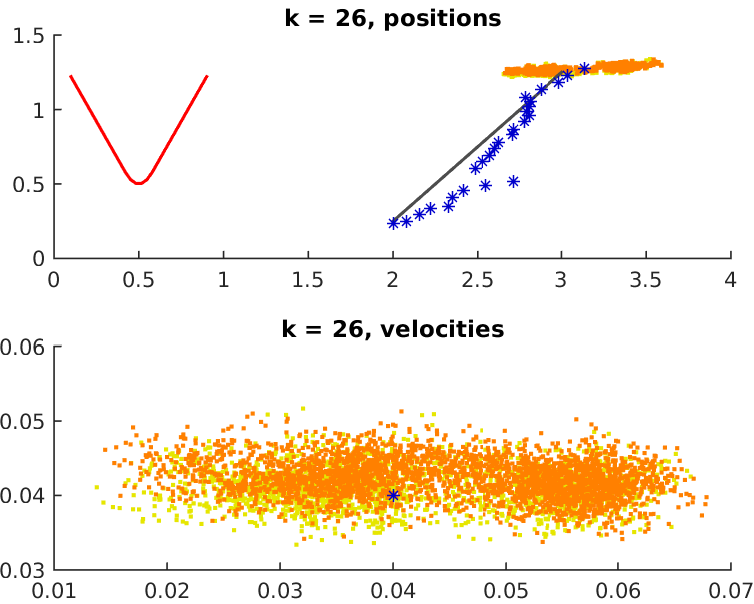
\includegraphics[width=0.5\textwidth]{img/q4_26.png}
\end{center}
  

\end{itemize} 

%Q5
\chapter{Improving the results using a post-regularised sequential Monte Carlo method}
\section*{Code}
As the fourth and fifth questions are both established on applying the algorithm~\ref{MonteCarlo}
to the submarine tracking problem, one decided to group the main code for questions 4 and 5
in the function \texttt{q4q5.m} ( \ref{q4q5}).\\
To call \texttt{q4q5} in the present case, one shall use \texttt{q51.m} and \texttt{q52.m} 
(to use it with the proper parameters, plot and save the results one can simply launch the script \texttt{plot\_q5.m}).\\
\lstinputlisting[caption={}]{../matlab_report/q51.m}
\lstinputlisting[caption={Question 5}]{../matlab_report/q52.m}
\section*{Results}
\begin{itemize}
\item Using the particle filter created previously\\
Due to the conception of the filter, the change of the number of distinct particles can only happen when resampling the set (ligne 57 of
\ref{MonteCarlo}) or at the prediction step (due to process noise, \ref{MonteCarlo}, l.78).
As $\sigma_a = 0$, there is no randomness in the prediction step, thus two indentical particles before this step will remain identical
after it. Therefore this step will not increase the diversity of particles.
The resampling step (with SIR filtering) takes the new particles directly from previous ones. Consequently, this step never
increases the number of different particles and often decreases it significantly, when some particles are more likely than others.
is equal to zero. Also, the change of bearing is small. Therefore, at this step,  the diversity of the particles can only decrease.
The effective number of particles is thus decreasing. One then looses the advantage of the particle filter, based on
the law of large numbers.\\
\begin{center}
 \includegraphics[width=0.66\textwidth]{img/q51.eps}
\end{center}
Taking a look at the results, one sees that the number of effective particles decreases exponentially with the number of steps.
This brings an error on the estimation of the target's position : the last three positions are off track whilst the previous three
were quite correct.

\item Using a regularized particle filter\\
By adding some noise in the resampling one can keep the number of effective particles near to the real number of particles,
using a post-regularized filter. Since the post-regularized filter adds noise to the particles, it may reduce the precision
of the estimation. Therefore, one only resamples when it is needed, which means when the effective number of particles becomes
smaller than a fixed threshold.
\begin{center}
\includegraphics[width=0.66\textwidth]{img/q52.eps}
\end{center}

On the plot, one observes that the post-regularized filter is efficient at keeping the effective number of particles high,
which makes the filter more reliable and effecient.
The estimated position is thus more precise with respect to the bearing (the distance with the observer is difficult to
estimate, and the post-regularization is not a magical solution here).
\end{itemize}
%Q6
\chapter{Analysing the error of the estimation}
\section*{Code}
One develops the Carmér-Rao lower bound and then the root mean square error for the submarine-tracking problem, using the
preceding codes :
\lstinputlisting[caption={Question 6}]{../matlab_report/q6.m}

\section*{Results}
\begin{center}
   \includegraphics[width=0.92\textwidth]{img/q6.eps}
\end{center}

At first, one finds that the experimental error (root mean square, RMS) is higher than the lower bound (Carmér-Rao lower bound,
CRLB), and they approximately follow the same course. They both diminish over time, meaning that the estimation converges towards a low variance. These results
 are promising.

Taking a closer look at the CRLB, at the begining the variance tends to augment because the observations do not give much
more information on the position than already available when the filter is started
(the bearing is close to constant). Starting at $k=6$, the change
of relative position is sufficient for the bearing to change more significantly, the variance then decreases.
When $k=15$, the observer makes a significant change of direction ; this gives information on the position of the
target, diminishing the variance ;  the CRLB diminishes substantially. In the end, after $k=20$, the change of bearing is again
close to constant and the acceleration close to zero, there is not enough noise in the system and as a result the CRLB augments
again.\\

From this, one can state that the quality of the estimation depends on two antagonistic effects : 
\begin{itemize}
\item the addition of entropy to the system by the random acceleration. This adds uncertainty on the
    state of observed process, and thus diminishes the quality of the available estimations.
\item the observation which gives information on the state of the system, reducing uncertainty,
    augmenting the precision of the estimator. When the bearing measurement the almost the same for
        a long time, new measures do not bring much new information, they are redundant.
\end{itemize}
Here there is no process noise, so the CRLB only diminishes, except at the beginning : at the firsts steps,
the uncertainty on the velocity is quickly decreasing while the uncertainty on the position increases a little bit
(thus the estimation of the whole state, including velocity, is getting better).\\


The empirical variance of the particle filter indicates that it is suboptimal, but not very far from the CRLB
(especially as the filter consider that $\sigma_a \neq 0$, one might maybe get a better estimation using
the information $\sigma_a = 0$).\\

As a suggestion of improvement, one could increase the number of particles in the system. It was asked to set it to 5000, 
by augmenting it we'd have to make more calculations but the variety of particles (the number of non redudant particles)
would stay higher, therefore enhancing the estimation.

\end{document}
